\chapter{Literature Review}
\section{Introduction}
Digital map has become an important role in our daily life. The modern digital map provides not only
geographic information, but also spatial services, like navigation, nearby restaurant
recommendation. All these services are supported by the spatial database.

There are two types of spatial database: euclidean space based and network space based. Network
space based database is widely used in traffic and transportation since cars must move
along the road network. Euclidean space based database is widely used in communication, because
signals transmit through the atmosphere. In this research project, all spatial queries
are euclidean space based.

There are mainly three kinds of query in classic
euclidean space based database: range, kNN (k-nearest neighbor) and RNN (reverse k-nearest neighbor).

\begin{figure}[htp]
\begin{subfigure}{.32\textwidth}
  \centering
  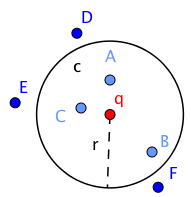
\includegraphics[width=.8\linewidth]{pic/rangeq.PNG}
  \caption{Range(q, r)=\{A,B,C\}}
\end{subfigure}%
\begin{subfigure}{.32\textwidth}
  \centering
  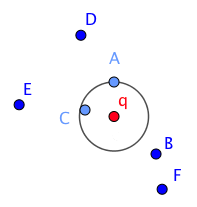
\includegraphics[width=.8\linewidth]{pic/knn.PNG}
  \caption{kNN(q, k=2)=\{A,C\}}
\end{subfigure}
\begin{subfigure}{.35\textwidth}
  \centering
  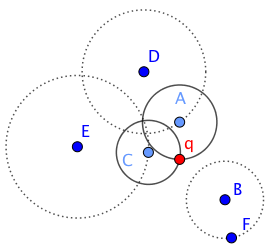
\includegraphics[width=.8\linewidth]{pic/rnn.PNG}
  \caption{RNN(q, k=1)=\{A,C\}}
\end{subfigure}
\caption{Three kinds of query}
\label{typeofquery}
\end{figure}

\begin{definition}{Range query:}
for a given query point $q$ and an range $r$, return an entity set:
$\{p | distance(p, q) <= r\}$. For example, in figure.\ref{typeofquery} (a), only $A,B,C$
will be retrieved because they are in the $circle(q, r)$.
\end{definition}

\begin{definition}{kNN query:}
for a given query point $q$ and an integer $k$, return an entity set:
$\{p | distance(p, q) <= distance(p_k, q)\}$, where $p_k$ is the k-th nearest neighbor of $q$.
For example, in figure.\ref{typeofquery} (b), $C$ is the 2rd nearest neighbor to $q$.
So the query only retrieve $A,C$ when $k=2$, and exclude all points further than $C$.
\end{definition}

There are two types of RkNN query:\@ monochromatic and bichromatic. We only introduce
monochromatic here, which is, both entities and query points belong to the same set.
In monochromatic RNN:\@ for a given query point $q$ and an integer $k$, return an entity set:\@ $\{p | q \in kNN(p)\}$.
For example, in figure.\ref{typeofquery} (c), when $k=1$, only $A,C$ will be retrieved, because $q$ is
$A$ and $C$'s nearest neighbor.

\begin{figure}[htp]
  \centering
  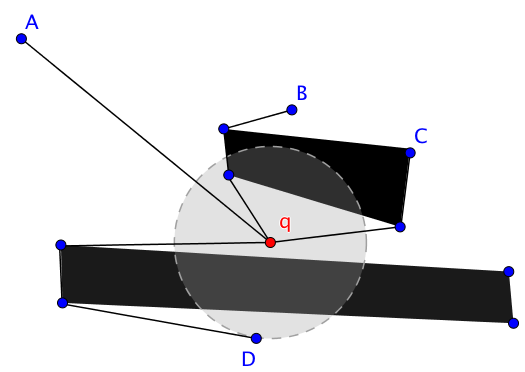
\includegraphics[width=0.8\linewidth]{pic/obs_dis.PNG}
  \caption{when obstacles exist}
\label{obs_dis}
\end{figure}

Traditional RNN has been well studied. Since they don't consider obstacles, the distance can be computed directly.
However, sometimes obstacles play an important role in the query. For example, there are many
restaurants in a large piazza, and restaurants want to know their competitors those who regard
them as the nearest neighbor. But there are many buildings, ponds and
rockwork in the piazza, so the query must consider these untraversable objects.

Query processing would be very different when obstacles exist, let's see a concrete example in
figure.\ref{obs_dis}:
The circle $c$ implies that $D$ is the nearest neighbor of $q$ in euclidean
distance, but because of the obstacles, $D$ becomes the furthest neighbor of $q$, so that
affected the result of range and kNN query;
also, the circle $c_2$ implies that $q$ is the nearest neighbor of $C$ in euclidean distance,
but $B$ is the nearest neighbor of $C$ based on obstacles distance, and this fact affected the
result of RNN\@. These obstacles distance based Range, kNN and RkNN queries are written as
$\mathit{OR, OkNN, ORkNN}$.

In section~\ref{lrsqp}, we are going to explore existing works on obstacles spatial queries.
$\mathit{ODC}$(\textit{Obstacles Distance Computation}), $\mathit{OR, OkNN, ORkNN}$ will be introduced. Each
subtopic will discuss pros/cons of existing works and identify the gap in these research.

In section~\ref{meshpf}, we are going to explore a new pathfinding framework. We will go
through all technical details of the framework, and discuss how it would speed up existing query
processing.

Finally we will come up with a possible direction for our research.

\section{Spatial Query Processing}\label{lrsqp}
% TODO: overview of this section

\subsection{Symbols And Formal Definition}\label{background}

All objects in database are represented by $T$; objects that we are interested in are
called entity, represented by $E$; objects that can block path are called obstacles,
represented by $O$. Formal definition of spatial query are:

\begin{definition}{obstacle range query (OR):}
given $E,T$, query point $q$,  and number $r$, 
  return $\{p | p \in E, d_o(p, q) <= r\}$.
\end{definition}

\begin{definition}{obstacle kNN query (OkNN):}
given $E,T$, query point $q$, and integer $k$,
  return $\{p | p \in E, d_o(p, q) <= d_o(p_k, q)\}$.
\end{definition}

\begin{definition}{Obstacle monochromatic RkNN query (ORkNN):}
given $E,T$, query point $q, q \in E$,
    return $\{p | p \in E, q \in OkNN(p)\}$.
\end{definition}

All math notations can be referred from table.\ref{notations}.
\begin{table}[ht]
\centering
\caption{Notations}
\begin{tabular}{|l|l|}
\hline
$d_e(p, q)$         & Euclidean distance from $p$ to $q$  \\
\hline
$d_o(p, q)$         & Obstacle distance from $p$ to $q$ \\
\hline
$sp(p, q)$          & shortest obstacle distance based path from $p$ to $q$, $d_o(p, q)=|sp(p,q)|$\\
\hline
$circle(q, r)$      & Circle with center $q$ and radius $r$ \\
\hline
$NN(q) / kNN(q)$    & (k) Nearest neighbor of $q$ based on euclidean distance \\
\hline
$iNN(q) / ikNN(q)$  & Incremental (k) nearest neighbor of $q$ based on euclidean distance \\
\hline
$mindist(node, q)$  & The minimal distance from point $q$ to a r-tree node \\
\hline
\end{tabular}
\label{notations}
\end{table}
\subsection{Spatial Indexing}\label{spatial_index}
%300
Objects in spatial query are regarded as stationary object, that is, they have a location and
don't move. For example, hospital and apartment are stationary objects, while car and mobile
phone are not. To retrieval these stationary objects effectively, we must use spatial
indexes. There are many kinds of spatial indexes, but in this section, we will only introduce R-tree,
which is one of the most common spatial indexes.

\begin{figure}[htp]
  \centering
  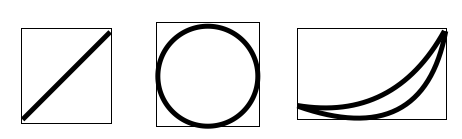
\includegraphics[width=.8\linewidth]{pic/mbr.PNG}
  \caption{MBRs}
\label{mbr}
\end{figure}

\begin{figure}[htp]
  \centering
  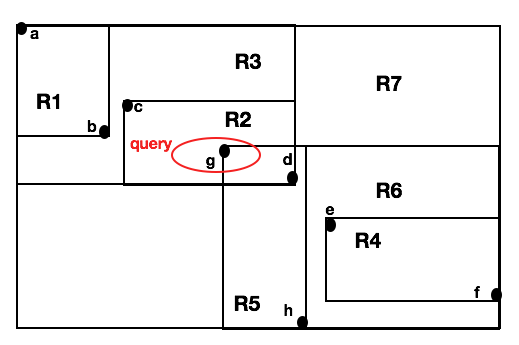
\includegraphics[width=0.8\linewidth]{pic/hierarchy_mbr.PNG}
  \caption{Hierarchy of MBRs}
\label{hierarchy_mbr}
\end{figure}

\begin{figure}[htp]
  \centering
  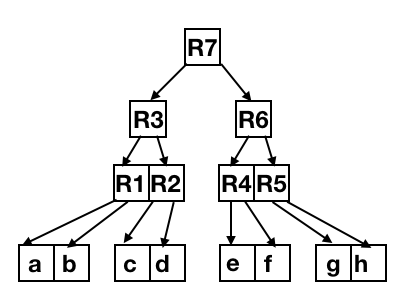
\includegraphics[width=0.8\linewidth]{pic/rtree.PNG}
  \caption{Tree structure}
\label{rtree}
\end{figure}

R-tree is a height-balanced tree \cite{guttman1984r}, all objects are stored in leaf node, and all interior nodes
contain either leaf node or descendant interior nodes. In leaf node, if an object is not a
point, it would be represented by its MBR (Minimal Bounding Rectangle),
for example, in figure.\ref{mbr}, both segments,
circle and irregular shape are represented by their MBR\@.
To guarantee efficiency, each non-root node of R-tree can contain at least $m$ entries and at
most $M$ entries, where $M$ is a constant when R-tree is built and $2<=m<=\lceil M/2\rceil$m
and the root node of R-tree alway has 2 entries.

Let's see a concrete example in
figure.\ref{hierarchy_mbr}:\@ $a,b,c,d,e,f,g,h$ are objects, $R1,R2,R5,R4$ are leaf-nodes, $R3,
R6$ are interior nodes, and $R7$ is the root; and figure.\ref{rtree} shows the corresponding
tree. Usually, objects retrieval start from the root, then narrow down to child node according
to spatial information in MBR, and finally retrieve objects from leaf-nodes. For example, in
figure.\ref{hierarchy_mbr}, the red oval is a range query, the retrieval progress is:

\begin{itemize}
  \item 1. Start from root node $R7$, and check all children nodes;
  \item 2. Since MBR of $R3$ contains query area, we will go to $R3$;
  \item 3. In $R3$, only $R2$ contains query area, so we will go to $R2$;
  \item 4. $R2$ is the leaf-node, so we can retrieve object in query area, which is $d$;
  \item 5. $R6$ also contains query area, so we will go to $R6$, then $R5$, and finally find
    that nothing needs to be retrieved;
\end{itemize}

Notice that in the example, to simplify the problem, all objects are point, but in practice,
they can be points and MBRs of any shapes, entities and obstacles may be stored in same R-tree.
Also notice that in retrieval progress, overlapping area may be explored multiple times, so there is a
variant of R-tree doesn't allow overlapping in interior node, called
$R^+$-tree\cite{sellis1987r+}.

There are many other variants to the traditional R-tree, they
improved efficiency in some aspects, but they still provide similar operations, so we only
introduce R-tree and the retrieval operation in this section, more details are in
\cite{guttman1984r}, \cite{beckmann1990r}, \cite{sellis1987r+}, \cite{kamel1993hilbert}.

Another important query in R-tree is Nearest Neighbour (NN) query. Since all nodes are organized by
their spatial information, NN can be easily retrieved by a kind of depth-first search (DFS), for example
if we want to find the NN of point $b$ in the figure.\ref{hierarchy_mbr}:

\begin{itemize}
  \item 1. Start from $R7$, since the MBR of $R3$ is the closest child to $b$, $R3$ should be visited first;
  \item 2. At $R3$, since $R1$ is the closest child to $b$, $R1$ should be visited first;
  \item 3. At $R1$, we find object $a$ and regard $a$ as a candidate, then we back to the parent node ($R3$);
  \item 4. At $R3$, the second closest child $R2$ should be visited;
  \item 5. At $R2$, we find object $c$, since $c$ is closer than $a$, $c$ should be current candidate,
  then we back to parent node;
  \item 6. Keep backtrack to parent node until return to $R7$, then visit next unvisited children;
  \item 7. At $R6$, the second closest child is $R6$, but $R6$ is further than current candidate $c$,
  so it won't be visited;
  \item 8. There no other nodes can be visited, so algorithm terminate and return the current candidate $c$;
\end{itemize}

Such NN query processing can be easily extended to kNN and ikNN (incremental kNN), here
$\mathit{ikNN(q)}$ can retrieve the nearest neighbor of $q$ incrementally,
for example, the first time call $\mathit{iNN(q)}$ will
retrieve the closest neighbor of $q$, and next time call $iNN(q)$ will retrieve the second
closest neighbor of $q$, and so on, $\mathit{ikNN}$ will be employed by some obstacle query processing,
see detail in section\ref{qp}.

\subsection{Obstacle Distance Computation}\label{odc}
%300
Obstacle distance between pair of point $p,q$ is the length of the shortest path from $p$ to $q$
without cross any obstacle. Obstacle distance computation (ODC) is a function that given
source point $q$ and target point $p$, return $d_o(q, p)$.
Before introducing more detail about ODC, we need to know some concepts.

\begin{itemize}
  \item \textit{Visibility graph:} visibility graph is a graph that edge exists between any pair of
vertexes if there are no obstacles between them. See example in the figure.\ref{vg}.
  \item \textit{Explored area}. The area is defined by $circle(q, r)$, all objects in this area
    have been retrieved from R-tree.
  \item \textit{Real path}. It's a path that all vertexes and edges of the path are in explored
    area, the length of path is the actual obstacle distance.
  \item \textit{Pseudo path}. It's a path that some part of it beyond the explored area.
  \item \textit{Euclidean lower-bound}: $d_o(p, q) >= d_e(p, q)$.
\end{itemize}

The obstacle distance of two points is the length of their shortest path in \textit{VG}.
Thus, the first step for ODC is to build VG, however, VG building is expensive, and can't fit
into main memory. Thus, existing ODC won't build global VG, instead, they will begin with
an explored area and build visibility graph based on that, called local visibility graph (LVG).

\begin{figure}[htp]
  \centering
  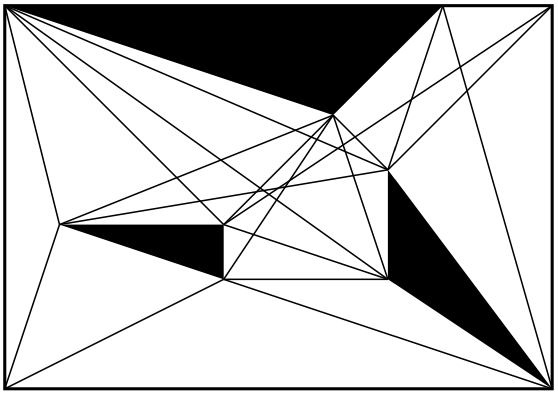
\includegraphics[width=.5\linewidth]{pic/vg.png}
  \caption{Visibility graph}
  \label{vg}
\end{figure}

Zhang proposed an ODC algorithm in 2004 \cite{zhang2004spatial}, for given pair of points
$p,q$, the algorithm will:

\begin{itemize}
  \item 1. At beginning, the radius of explored area is $r=d_e(p,q)$;
  \item 2. Retrieve all obstacles in $circle(q, r)$, and build LVG;
  \item 3. Compute the shortest path from $q$ to $p$ based on this LVG;
  \item 4. If $d_o'(p, q) > r$, enlarge the explored area to $r=d_o'(p, q)$, go to step2;
  \item 5. Otherwise the algorithm terminates because $d_o'(p, q)$ must be the length of a real path;
\end{itemize}

Let's see an example in the figure.\ref{edbt_odc}. At beginning, the radius of explored area is
$r=d_e(p, q)$, so $o_1,o_2$ will be retrieved, because they are in $circle(q, r)$; then LVG
will be built and a temporary obstacle distance $d_{o1}(p, q)$ will be computed; but we can't
guarantee that $d_{o1}(p, q)$ is the length of real path ($d_{o1}(p, q) > r$), so we
must set $r=d_{o1}(p, q)$ to enlarge the explored area; then $o_3, o_4$ will be retrieved, the
LVG will be updated and $d_{o2}(p, q)$ will be computed; the algorithm will continue and the
explored area will be updated until the explored area is large than the temporary obstacle
distance.

\begin{figure}[htp]
  \centering
  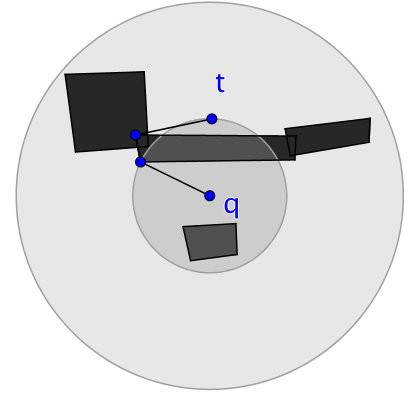
\includegraphics[width=.5\linewidth]{pic/edbt_odc.png}
  \caption{example of ODC in Zhang's work}
  \label{edbt_odc}
\end{figure}


The correctness of the terminate condition can be easily proofed:  if $d_o(p, q) <= r$, because of
the \textit{Euclidean lower-bound} all vertexes must be in $circle(q, r)$, so $d_o(p, q)$ is the length of real path.

Xia also proposed a similar ODC algorithm in same year \cite{xia2004fast}. The different part
is that Xia's algorithm only retrieval obstacles on the path, if obstacles exist,
LVG will be updated and shortest path will be re-computed, otherwise the algorithm terminated.
Let's see an example in the figure.\ref{bncod_odc}. In the first iteration, obstacle $b1, b2$ will
be retrieved because they are on the segment $qp$ , then compute shortest path $r$; in the
second iteration, $b3$ will be retrieved, then LVG will be updated and shortest path will be
re-computed because $b3$ is on the shortest path of previous iteration. The algorithm will
be terminated in the second iteration because there are no obstacles on the new shortest path.
\begin{figure}[htp]
\begin{subfigure}{.5\textwidth}
  \centering
  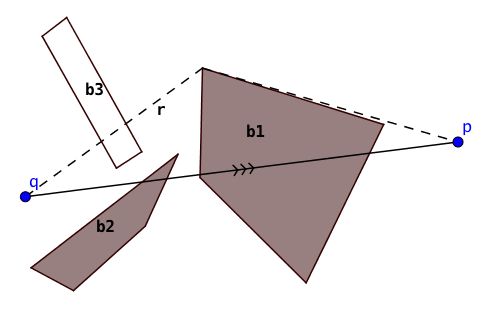
\includegraphics[width=.8\linewidth]{pic/bncod_odc1.PNG}
  \caption{the first iteration}
\end{subfigure}%
\begin{subfigure}{.5\textwidth}
  \centering
  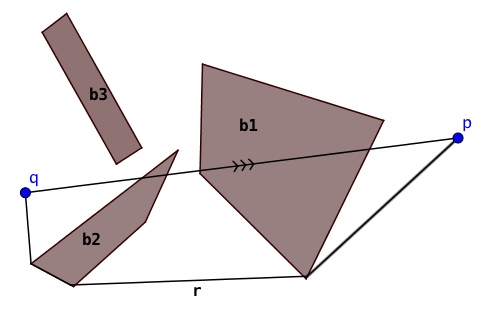
\includegraphics[width=.8\linewidth]{pic/bncod_odc2.PNG}
  \caption{the second iteration}
\end{subfigure}
\caption{example of ODC in Xia's work}
\label{bncod_odc}
\end{figure}
\subsubsection{Discussion of ODC}
We can see that less obstacles will be involved in Xia's ODC algorithm, for example, if we run Xia's algorithm
on the case in the figure.\ref{edbt_odc}, $o_2$ would never be retrieved. Thus, for a pure obstacle
distance query, Xia's algorithm is better than Zhang's. But the conclusion may not be true for other
spatial queries, and this will be discussed in section.\ref{qp}.

\subsection{Range and kNN Query Processing}\label{qp}

Range query processing is quite straightforward, following obstacle range query processing has
been proposed in Zhang's work \cite{zhang2004spatial}:
\begin{itemize}
  \item 1. Build LVG for explored area $circle(q, r)$, where $q$ is the query point and $r$ is the range;
  \item 2. Run Dijkstra on LVG, all entity $p$ that $d_o(p, q) <= r$ will be retrieved;
\end{itemize}
The correctness of range query can be proofed by \textit{Euclidean lower-bound} property.
Both Zhang and Xia has proposed obstacle query processing for kNN in their work, and since they are under
the same framework, we will only discuss Xia's obstacle kNN query:
\begin{itemize}
  \item 1. Retrieval euclidean kNN $p_1, p_2, \cdots p_k$, and initialize a heap with \\
  $\{d_o(p_1, q), \cdots d_o(p_k, q)\}$, and assume in the heap: $d_o(p_i,q)<=d_o(p_{i+1}, q)$;
  \item 2. Retrieval next euclidean NN $p'=iNN(q)$;
  \item 3. If $d_o(p',q)<d_o(p_k, q)$, replace $p_k$ by $p'$ in the heap and go to step 2;
  \item 4. Otherwise if $d_e(p', q) >= d(p_k, q)$, terminate algorithm;
\end{itemize}
Let's proof the correctness. Firstly, the algorithm will terminate in finite steps because
$d_e(p', q)$ keep increase and $d_o(p_k, q) $ keep decrease; secondly, when algorithm
terminated, all entities in heap are entities need be retrieved, otherwise there is a $p_x$
s.t $d_o(p_x, q) < d_o(p_k, q)$, because of \textit{Euclidean lower-bound} property we have
$d_e(p', q) <= d_o(p', q) <= d_o(p_k, q)$, so $p_k$ must has been replaced by $p_x$, so it's
impossible.

\subsubsection{Discussion of Range and kNN Query Processing}\label{disknn}
It is worth to notice that, in range and kNN, we need to compute multiple pairs of obstacle distance with same
source $q$, so Zhang's ODC algorithm can be more efficient than Xia's ODC algorithm.
The reason is that Zhang's algorithm will compute single source shortest path for LVG,
while Xia's algorithm only computes single pair of shortest path, so information can't be resued when destination changed.

Also we can summarize three problems in the range and kNN query processings.

Firstly, they will compute pseudo path during iteration, and pseudo path will cause redundant
computation. For example, in figure.\ref{edbt_odc}, pseudo paths in each iteration are
completely different, and the LVG has been revised. Notice that revising is changing things
already exist, which may cause redundant computation.

Secondly, sometimes the algorithm can terminate earlier without end up with a large explored
area. For example, in figure.\ref{tighter}, the current explored area is $circle(q, r)$, and
the current path is already a real path, but the algorithm will continue until the explored
area become $circle(q, r_2)$, where $r_2=d_o(q, p_k)$.
\begin{figure}[htp]
  \centering
  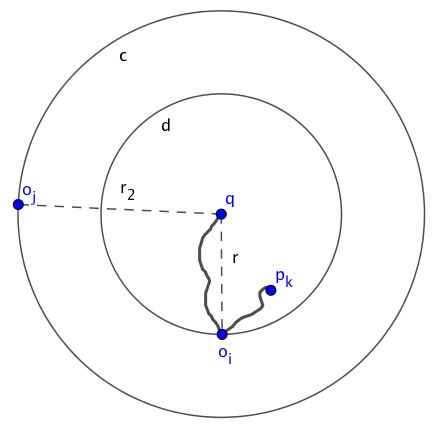
\includegraphics[width=.5\linewidth]{pic/tighter.png}
  \caption{Unnecessary explored area}
  \label{tighter}
\end{figure}

Thirdly, searching order of kNN is inefficient. Both Zhang and Xia's kNN query processing 
choose the next candidate by $p=iNN(q)$, which is based on euclidean distance,
while, $p$ may not be the next nearest neighbor of $q$ in obstacle distance.

From three observation above, we can conclude three ways to improve ODC algorithm. First, we
can only compute real path and enlarge explored area incrementally, in another word, we 
add new things to LVG rather than revise it. Second, we can define a tighter terminate
condition. Third, we need an incremental obstacle kNN (iOkNN) algorithm.

\subsection {Monochromatic Obstacle Reverse k-Nearest Neighbor ($\mathit{ORkNN}$)} \label{RNN}

A native query processing for $\mathit{ORkNN}$ is running $kNN$ query for each entity, but this approach is
too slow, so pruning is necessary.
In 2011, Gao proposed a heuristic pruning called \textbf{\textit{boundary pruning}}
\cite{gao2011efficient}. Before discussing detail of $\mathit{ORkNN}$, let's introduce some
concepts, and to simplify problem, let's assume $k=1$.
\begin{definition}{(Boundary point/ Boundary Set)}
  Given a point $p \in E$, a vertex $v$ of obstacle $o \in O$, and a query point $p \in E$,
  $v$ is boundary point to $(p, q)$ iff $d_o(p, v) < d_o(q, v)$, where $v$ can be any point in
  space exclude obstacles.
  All boundary vertices formed boundary set $B$.
\end{definition}

\begin{definition}{(Point Angle)}
  Given a point $p \in E$, a query point $q$ and let $q$ be the origin. The point angle of
  $p,q$ is $\angle Xqp$ where $X$ can be any point right to the $q$ and on x-axis, write as
  $\theta_{p}$.
\end{definition}

\begin{lemma}
Given a query point $q$,
a current candidate point $p$, and another candidate $p'$, both $q,p,p' \in E$,
if $v$ is boundary vertex of $(p,q)$, and $sp(q, p')$ cross $sp(v, p)$ at some point $x$,
then $d_o(q, p') > d_o(p, p')$ so that $p'$ can be pruned.
\label{bplemma}
\end{lemma}
\begin{proof}
Because $sp(q, p')$ cross $sp(v, p)$ at $x$,
therefore $d_o(q, p') = d_o(q, x) + d_o(x, p')$;
because the definition of \textit{boundary point},
therefore $d_o(q, x) > d_o(p, x)$,
so we have $d_o(q, x) + d_o(x, p') > d_o(p, x) + d_o(x, p') >= d_o(p, p')$
\end{proof}
However, lemma~\ref{bplemma} can't be applied directly on pruning,
because under existing framework, it's computationally expensive to determine whether such $x$ exist
for given $q, p, p'$. Thus Gao proposed an approximate pruning instead:

\begin{definition}{Boundary Region Pruning (BRP):}
  Given a query point $q \in E$, a candidate point $p \in E$, let $v_{min}$ be the boundary
  vertex of $p$ with the minimal point angle, let $v_{max}$ be the boundary vertex of $p$
  with the maximal point angle, and let $d_{max}$ be the maximal euclidean distance from $q$ to any
  point along $sp(q, v_{min}), sp(q, v_{max})$; for any $p' \in E$, if
  $\theta_{p'} \in [\theta_{v_{min}}, \theta_{v_{max}}]$ and $d_e(p', q) > d_{max}$, then
  $p'$ will be pruned.
\end{definition}

Let's see how does \textit{BRP} work from a concrete example in figure.\ref{bp}. In this case,
$v_{max}, v_{min}$ are $a, b$ respectively, and $\theta_{p'} \in [\theta_{v_{min}},
\theta_{v_{max}}]$. The \textit{BRP} assumes that $sp(q, p')$ is very likely cross segment
$[a, p]$ or $[b, p]$, so that be pruned. We can use the arc to represent segment $[a, p]$ and $[b, p]$ approximately,
so that we only need to test angle and euclidean distance in the pruning. As we've applied many
approximations, the pruning approach introduced false miss, but according to experiments, the
false miss rate is only 0.05 which is acceptable.

\begin{figure}[htp]
  \centering
  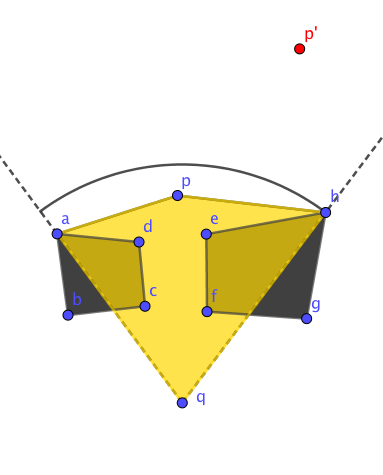
\includegraphics[width=.4\linewidth]{pic/bp.png}
  \caption{Boundary Region Pruning}
  \label{bp}
\end{figure}

The entire framework of $ORNN$ query processing has two stage,
the first stage is \textit{Filter}:
\begin{enumerate}
  \item Initialize heap with root node of R-tree, the key is $mindist(root, q)$;
  \item Retrieve top entry $c$ from heap;
  \item If $c$ has been pruned, go back to 2;
  \item If $c$ is interior node, push children to heap;
  \item If $c$ is an entity point, add $c$ to candidate set, call $ODC(q, c)$ to find boundary
    point set, and call $BRP$ to pruning search space, finally go back to 2;
\end{enumerate}

The second stage is \textit{Refinement}: run $ONN$ on each point in candidate set, and only keep those
candidates who regard $q$ as their nearest neighbor.

In 2016, Gao extended the query processing to $\mathit{ORkNN}$\cite{gao2016reverse}. Instead of being
removed immediately, in $\mathit{ORkNN}$ query processing, a node will be removed only if it has been
pruned k times, because it implies that
$\exists p_1, p_2,\cdots p_k$ satisfy:
$$
d_o(p_1, p') < d_o(q, p'), d_o(p_2, p') < d_o(q, p'),
\cdots d_o(p_k, p') < d_o(q, p')
$$
so $q$ can't be k-nearest neighbor of $p'$.

Gao also noticed that it is more practical to only consider a bounded area. For example,
it's not necessary to consider objects in Sydney when query point is in Melbourne. Thus,
researchers proposed two variations of $\mathit{ORkNN}$: $\delta$\textit{-ORkNN} which is constraint search space by obstacles
distance and $\mathit{CORkNN}$ which is constraint search space by a region.

\subsubsection{Discussion of $\mathit{ORkNN}$}\label{disorknn}
There are still some problems in current $\mathit{ORkNN}$ query processing.

Firstly, same as problem in $\mathit{OkNN}$, the algorithm explores search space in order of euclidean
distance. To solve this problem, an $\mathit{iOkNN}$ algorithm is necessary.

Secondly, it employed $ODC(q, c)$ in query processing. As we've discussed in
section~\ref{disknn}, $ODC(q, c)$ can't reuse computed information.
Also we should notice that \textit{boundary pruning} works on any path, not just shortest path.
So \textit{boundary pruning} can also be applied on $ODC$, but current framework doesn't
support this. To solve this problem, we need to redesign an $ODC$ algorithm for $\mathit{ORkNN}$ query processing.

Thirdly, it's hard to utilize preprocessing under this framework.
On the one hand, the query processing relies on
\textit{BRP}, but it is query sensitive according to definition; On the other
hand, for whatever kinds of preprocessing, \textit{ODC} would be involved, and it may cause
building global visibility graph which is expensive. The former can be
solved by redefining \textit{Boundary point}, while the latter can't be solved under current
framework, so we need a new framework for \textit{ODC}, section~\ref{meshpf} will introduce a
possible framework to solve this problem.

\section{Literature Review of Pathfinding On Navigation Mesh}\label{meshpf}
Because of the limitation of visibility graph, navigation mesh comes to our sight. Navigation mesh
is a kind of spatial decomposition. It divided traversable space into convex polygons, and these
polygons are called mesh. The figure.\ref{nav} shows an example.
\begin{figure}[h]
  \centering
  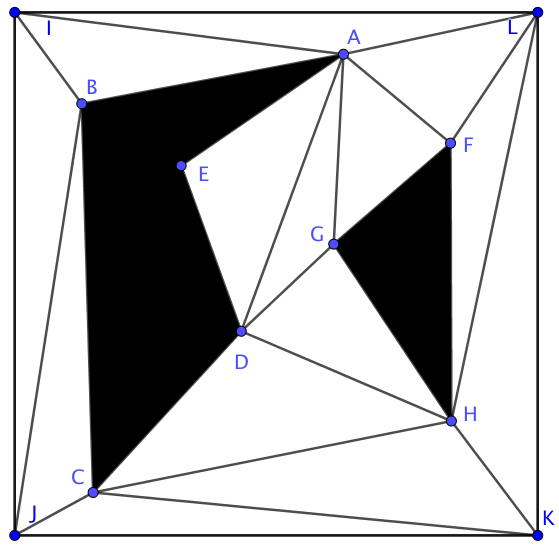
\includegraphics[width=.5\linewidth]{pic/nav.png}
  \caption{Navigation mesh}
  \label{nav}
\end{figure}
Compare to visibility graph, navigation mesh can be generated by triangulation, which is much
faster, besides, it has less number of edges and can be easily modified. It seems like a
perfect framework for ODC.

Navigation mesh used to be not suited for spatial database scenario. Ronald first proposed this
concept in 1986 \cite{ronald1986pathfinding}, then it is applied on robotics and game
pathfinding, three widely used algorithms are:

\begin{itemize}
  \item Channel Search \cite{kallmann2005path}: first find an abstract path from start to target
    composed by polygons, then refine the abstract path to a sequence of concrete points. This
    algorithm only generate an approximately shortest path, the lack of optimality makes it not
    suit for kNN query.
  \item TA* \cite{demyen2006efficient}: similar to Channel Search, but it can repeat the search
    process until finding an optimal shortest path. The repeating is time-consuming, so it is not
    suited for query processing.
  \item TRA* \cite{demyen2006efficient}: similar to TA*, but TRA* can utilize preprocessing to
    speed up pathfinding. The problem is that the precomputed information will be invalid when
    environment change, so it is not suited for database scenario.
\end{itemize}

But the fact has been changed by a recent work called \textbf{Polyanya} \cite{cuicompromise}.
It is a fast, optimal and online pathfinding algorithm which is perfect for
query processing in the spatial database.

\subsection{Polyanya}\label{polyanya}

Similar to other pathfinding algorithms, Polyanya has three components:

\begin{itemize}

  \item Search Nodes: different from other algorithms, they are not concrete nodes. A search
    node $(I, r)$ is a tuple of segment $I=[a, b]$ and root $r$. The segment is on the edges of
    mesh, the root is a point and all points on the segment are visible from the root.
    The figure.\ref{snode} shows an example of search node.

   \begin{figure}[h]
     \centering
     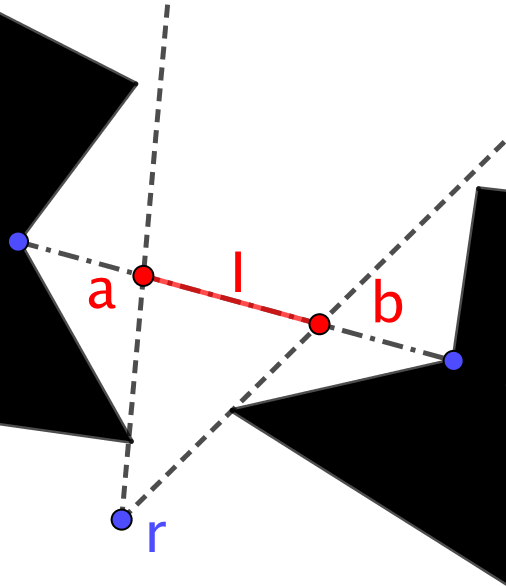
\includegraphics[width=.2\linewidth]{pic/snode.png}
     \caption{Search Node}
     \label{snode}
   \end{figure}

  \item Successors: a successor of a search node $(I, r)$ is also a search node $(I', r')$.
  Push $(I, r)$ away from $r$ and through the interior of an adjacent traversable polygons,
  successors are found on the perimeter of these polygons(from \cite{cuicompromise}).
  If $I'$ is not visible from the original root $r$, $r'$ has to change to an end-point of $I'$, which is called
  \textit{Non-observable successors}; otherwise $r'=r$, which is called \textit{Observable
  successors}. For example, in the figure.\ref{suc},  $([z,g],r), ([g,f],r), ([f,y],r)$
  are observable successors, and $([b,c],b),([c,d],b),([d,e],b),([e,y],b)$ are non-observable
  successors.

    \begin{figure}[h]
      \centering
      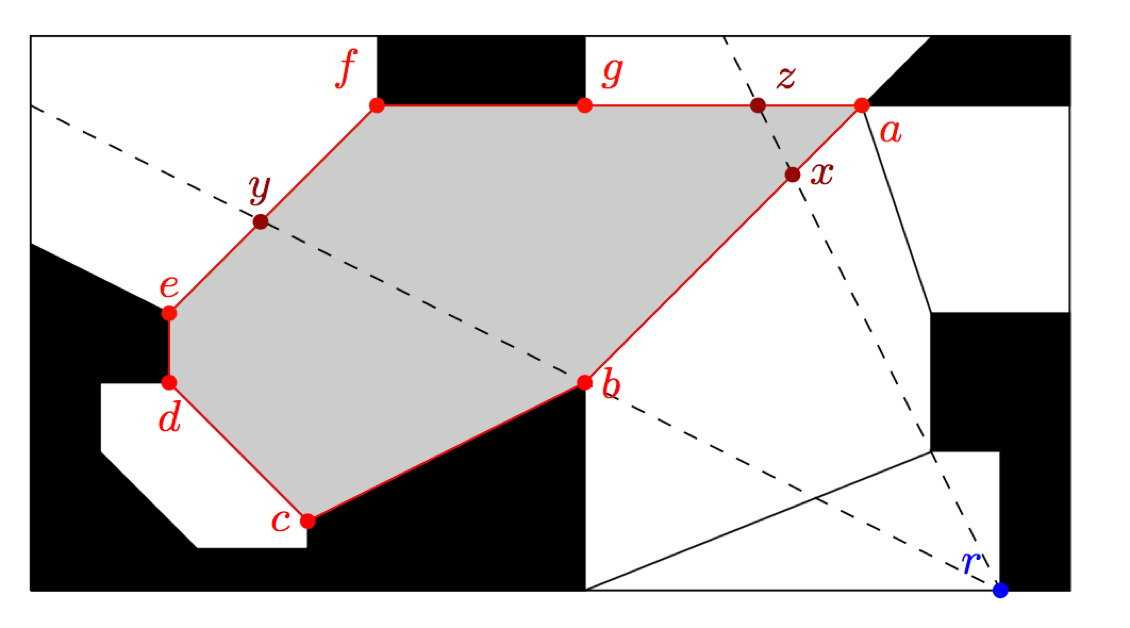
\includegraphics[width=.6\linewidth]{pic/suc.png}
      \caption{Successors of $([b,x],r)$}
      \label{suc}
    \end{figure}

  \item Evaluate Function: to determine the priority of the search node. It has three parts:
    \textit{g-value} which is the length of shortest path from start to root;
    \textit{h-value} which is estimated lower-bound of distance from $r$ to target through $I$;
    \textit{f-value=g+h} which is the key of search node in the priority queue. The computation for
    \textit{h-value} depend on relative location between root and target, let's see an example in
    figure.\ref{ef}:

    \begin{figure}[htp]
      \centering
      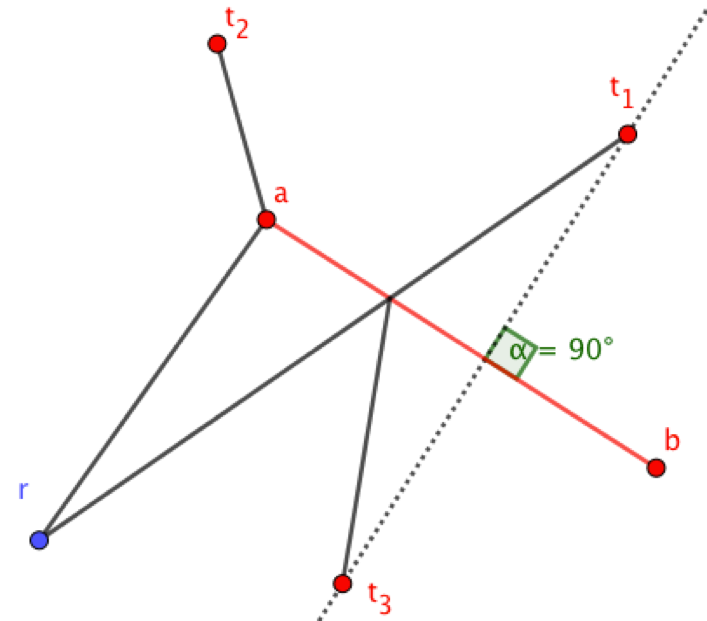
\includegraphics[width=.4\linewidth]{pic/ef.png}
      \caption{Three possible target locations for $([b,x],r)$}
      \label{ef}
    \end{figure}

    \begin{itemize}
      \item If the target is $t_1$, segment $[r, t_1]$ cross segment $[a,b]$, the
        \textit{h-value} in this case is the euclidean distance.
      \item If the target is $t_2$, at the opposite side of $r$ but $[r, t_2]$ doesn't across
        $[a,b]$, the \textit{h-value} is the sum of euclidean distance from one of end-point to $r$
        and $t_2$.
      \item If the target is $t_3$, at the same side of $r$, we can use its mirror through
        $[a,b]$, so it may become $t_1$ or $t_2$.
    \end{itemize}
\end{itemize}
The pathfinding process of \textit{Polyanya} is similar to \textit{A*}: pop out search node with minimal
\textit{f-value} and generate successors until the terminate condition satisfied:
\begin{itemize}
  \item \textbf{Case 1:} the queue has been empty, which means no path exists;
  \item \textbf{Case 2:} the segment of search node is on the mesh that contains the target,
    which means a path has been found.
\end{itemize}
Because the \textit{f-value} of search node in \textbf{Case 2} is the actual distance (not
the lower-bound), it corresponding to the shortest path.

\subsubsection{Discussion of Polyanya}
\textit{Polyanya} is an \textit{A*} algorithm that only computes shortest path for a single pair
of points. But it can be naturally extended to single source algorithm by setting
\textit{h-value} to be the distance from root to the segment. The revised \textit{Polyanya} can be
used on incremental kNN query processing.

\section{Proposed Research}
Consider advantages of navigation mesh, we are goin to get ride of visibility graph and design navigation mesh based approaches.
My research will improve obstacle queries processing in following directions: spatial indexing,
preprocessing, and simplification.

\subsection{Improve Spatial Indexing}
We can combine navigation mesh pathfinding with R-tree indexing, so that we can answer the
\textit{OkNN} query in one pass and reduce the number of node access.
Existing works are doing pathfinding and objects retrieval separately, so they have to do
R-tree operation multiple times, while R-tree is disk-based in practice, and node access can be
the bottleneck. In 2004, Xia proposed unified R-tree \cite{xia2004fast}, that is, storing data
points and obstacles together, and it turns out that unified R-tree is more efficient in
\textit{OkNN} query processing. Thus, combining pathfinding with R-tree may make further
improvement.

\subsection{Make Preprocessing Possible}
It is possible to design a navigation mesh flood-fill algorithm based on \textit{Polyanya} so
that for each entity we can compute the distance to its neighbor (not necessary to be the
nearest), and use this information in pruning. The complexity of this processing is constraint
by the number of edges, and because of the Euler Characteristic in planar: $V-E+F=2$, the
complexity should be acceptable.

\subsection{Improve Pruning}
As we've discussed in section.\ref{disorknn}, boundary pruning works on any path, so that we can
employ this technique in revised \textit{Polyanya}. To be more specific, when generating
successors, we can ignore those successors who have crossed any boundary. In doing so, there
are no approximations, so the pruning will be not only efficient but also accurate.

\subsection{Simplification}
We can simplify mesh and obstacles.

\begin{figure}[h]
  \centering
  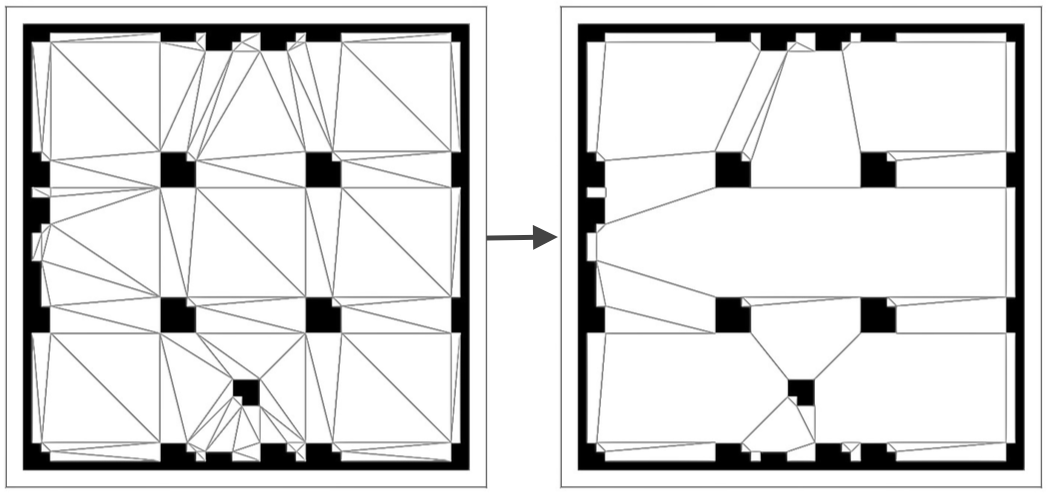
\includegraphics[width=.8\linewidth]{pic/merge.png}
  \caption{Merged navigation mesh\cite{cuicompromise}}
  \label{merge}
\end{figure}

To simplify mesh, we can merge them while retaining convexity. For example, the figure.\ref{merge}
shows a greedily merged navigation mesh.

To simplify obstacles, we can replace them by their convex hull.
Existing works represent obstacles by their MBRs because storing
original shape of obstacles is expensive and will increase the cost of
building visibility graph. But it is not a problem for navigation mesh, so we use their
original shape to improve the accuracy. But we can still simplify them without the loss of accuracy.
Let's see an example in the figure.\ref{convex}, the blue polygon is the original shape of
the obstacle, its convex hull is $ABCDE$, and grey pieces are complement area:
\begin{figure}[h]
  \centering
  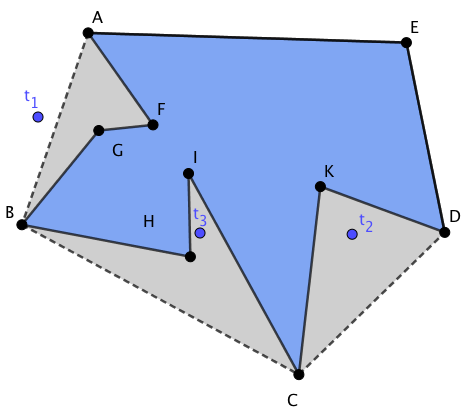
\includegraphics[width=.6\linewidth]{pic/conv.png}
  \caption{Replace by convex hull}
  \label{convex}
\end{figure}
\begin{itemize}
  \item If the location of the target is $t_1$, which is out of the convex hull, the shortest path
    would never pass the complement area
  \item If the location of the target is $t_2$, which is in the complement area but still visible
    from the perimeter, the shortest path can still be found when the segment of a search node
    reaches the perimeter.
  \item If the local of the target is $t_3$, which is in the complement area but not visible from
    the perimeter, we can precompute the shortest path from $t_3$ to some visible vertices, in
    this case is $H$.
\end{itemize}
Because of the Euler Characteristic,
simplification can reduce the scale of problem significantly for navigation mesh based
approaches.

\section{Conclusion}
In this thesis, we've explored existing works related to obstacle spatial queries and discussed
their pros and cons. We also identified a new direction for research, which is navigation mesh
based obstacle spatial query. It may outcompete all existing visibility graph based approaches
by efficiency and accuracy.
